%!TEX root = ../master.tex
\section{3rd party app developer attacking the consumer}\label{3rdpartyattacktree}
Our smart meter system allows developers to create their own apps for displaying the smart meter data as well as control the connected appliances.
This makes it possible for the developer to handle the data of the consumer and thus makes it possible for a malicious developer to send the data back to himself.
The purpose of this could be to sell the information to information gatherers who are willing to buy the information as mentioned in \cref{informationGathererVsConsumer}.

The attack tree for the 3rd party app developer can be seen on \cref{information_stealing_tree}.
As the app has direct access to the smart meter data, it is easy for the developer to obtain the data and send it to a database through the platform that the application is installed on.
He can then choose to analyze the data and create a profile (this was discussed in \cref{informationGathererVsConsumer}).
At last he can sell the profile (or even just the raw data) to some information gatherer.

\afterpage{% Insert after the current page
\cleardoublepage
\thispagestyle{plain}
\KOMAoptions{paper=A3,paper=landscape}
\recalctypearea

\begin{figure}
  \begin{center}
    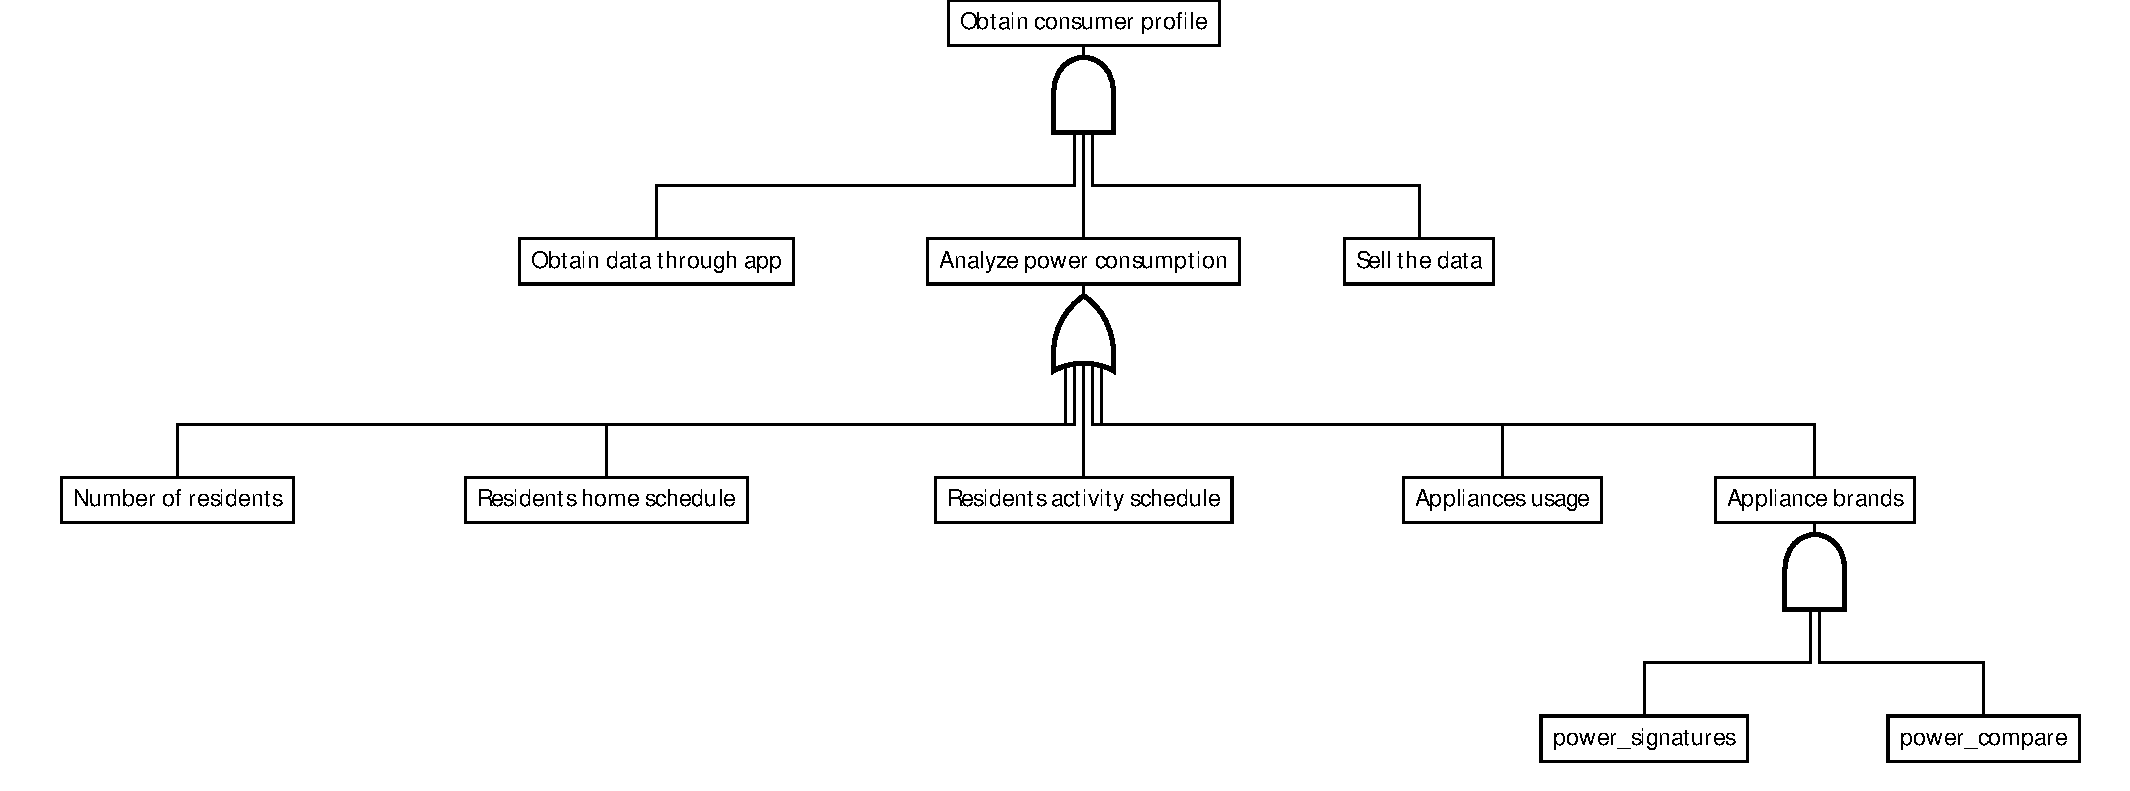
\includegraphics[width=\textwidth]{graphviz/3rd_party_vs_consumer.pdf}
  \end{center}
  \caption{A 3rd party app developer attacking the consumer through their app.}
  \label{3rdpartyTree}
\end{figure}

\cleardoublepage
\KOMAoptions{paper=A4,pagesize}
\recalctypearea
}

